\input{preamble.tex}
\usepackage{lmodern}

% --------------------------------------------------------------------
% --------------------------------------------------------------------
% ---- ENTER YOUR PROJECT DETAILS BELOW

% ---- title of the project
\title{Scalable ERA5 Analysis with Pandas and Dask}

% ---- names of team members
\author{
    \small Aditya Dahiya \and
    \small Adwita Joglekar \and
    \small Saachi Sirola \and
    \small Brajesh K. Mahto
    }

% ---- enter the team number below
\rhead{Team Dask-Pandas}

% --------------------------------------------------------------------
% --------------------------------------------------------------------


% --------------------------------------------------------------------
% --------------------------------------------------------------------
% ---- DO NOT CHANGE THIS BLOCK OF CODE
\begin{document}
\maketitle
% --------------------------------------------------------------------
% --------------------------------------------------------------------

\begin{abstract}
This report presents a case study on scaling ERA5 weather analysis from an
eager Pandas workflow to a chunked Dask workflow. We benchmark runtime and
memory, validate numerical parity, and analyze practical trade-offs in
chunking and execution strategy. Beyond performance, we include a focused
anomaly analysis for South Asia in 2024 and summarize implementation effort,
debugging complexity, and lessons for reproducible scientific data pipelines.
\end{abstract}



% --------------------------------------------------------------------
% --------------------------------------------------------------------
% ---- WRITE YOUR REPORT BELOW

\section{Introduction}
This project evaluates when Dask improves practical scalability for weather
reanalysis analysis compared to Pandas. We use ERA5 single-level data as a
high-dimensional case study with multiple variables, hourly time steps, and
spatial grids. The assignment objective is not only runtime comparison but also
understanding memory behavior, chunking effects, correctness parity, and
implementation trade-offs in real workflows.


\section{Related Work}
The project is grounded in established scientific-data workflows with NetCDF,
array-based regional reductions, and temporal aggregation. Rather than
introducing a novel algorithm, our contribution is an experience-driven
evaluation of scalable data processing choices in a realistic ERA5 pipeline,
including failure modes and revision steps.

\section{Our contribution}
We provide:
\begin{enumerate}
    \item A baseline Pandas workflow for a feasible subset and a larger South
    Asia run.
    \item An aligned Dask workflow that computes the same daily regional
    metrics for parity testing.
    \item A benchmark orchestrator that runs scripts end-to-end and exports
    runtime, peak memory, chunk-sweep, and consistency artifacts.
    \item A consolidated result layout in \verb|data/results/| split by
    \verb|central_india/|, \verb|south_asia/|, and \verb|benchmark/|.
\end{enumerate}

\section{Methods}
\subsection{Data}
Two ERA5 request profiles were used:
\begin{itemize}
    \item Compact consistent-slice request ($\sim$464 MB) for baseline
    Pandas analysis.
    \item Full 2024 request ($\sim$12 GB) for large-volume analysis and Dask
    scalability evaluation.
\end{itemize}

The analysis variables include near-surface temperature and radiation terms,
with daily statistics and anomaly comparisons.

South Asia was analyzed over approximately $5^{\circ}\mathrm{N}$--$35^{\circ}\mathrm{N}$
and $65^{\circ}\mathrm{E}$--$100^{\circ}\mathrm{E}$ with 6-hourly steps in 2024.

\subsection{Analysis pipelines}
\textbf{Pandas South Asia baseline.}
The Pandas workflow computes regional daily metrics (temperature, cloud,
radiation), derived quantities (net radiation), and anomalies from monthly
means.

\textbf{Dask aligned workflow.}
The Dask workflow uses lazy loading and chunked execution, then computes the
same daily metrics so that direct parity checks can be performed.

\textbf{Benchmarking.}
An orchestration script runs both workflows, records runtime and peak RSS
memory, sweeps chunk settings, and exports consistency tables.

\textbf{Anomaly definition.}
For each variable $x$ and month $m$, daily anomalies are computed as
\[
\text{anom}_{d,m} = x_{d,m} - \overline{x}_{m},
\]
where $\overline{x}_{m}$ is the within-2024 monthly mean for that variable.

\section{Results}
\subsection{Runtime and memory}
For the full-window South Asia benchmark:
\begin{itemize}
    \item Pandas recompute runtime: 13.04 s, peak RSS: 289.07 MB.
    \item Dask aligned runtime (chunk=96): 37.69 s, peak RSS: 428.04 MB.
\end{itemize}

Chunk sweep results for Dask (full-window):
\begin{itemize}
    \item chunk=24: 39.93 s, 447.02 MB
    \item chunk=48: 39.70 s, 438.93 MB
    \item chunk=96: 40.30 s, 442.30 MB
    \item chunk=192: 39.11 s, 439.80 MB
    \item chunk=auto: 25.67 s, 370.12 MB
\end{itemize}

The \verb|auto| chunk strategy performed best in both runtime and memory in
this environment.

\begin{table}[h]
    \centering
    \caption{Full-window benchmark summary (South Asia 2024)}
    \begin{tabular}{lcc}
        \hline
        Method & Runtime (s) & Peak RSS (MB) \\
        \hline
        Pandas baseline & 13.04 & 289.07 \\
        Dask aligned (chunk=96) & 37.69 & 428.04 \\
        Dask aligned (chunk=auto) & 25.67 & 370.12 \\
        \hline
    \end{tabular}
\end{table}

\subsection{Correctness and consistency}
Daily parity over 366 rows showed very small differences:
\begin{itemize}
    \item \verb|t2m_c| mean abs diff: $1.09 \times 10^{-6}$
    \item \verb|ssr| mean abs diff: $3.01 \times 10^{-6}$
    \item \verb|str_nlw| mean abs diff: $8.20 \times 10^{-7}$
    \item \verb|net_rad| mean abs diff: $1.09 \times 10^{-6}$
    \item \verb|tcc| mean abs diff: 0.0
\end{itemize}

Anomaly parity is also strong, with mean absolute differences in the
$10^{-6}$ range.

\subsection{Unexpected behavior and revision}
The initial Dask implementation exhibited counterintuitive performance
characteristics. When chunking the 12~GB ERA5 dataset with very small time
dimensions (\verb|valid_time=4| steps per chunk), we observed that total
runtime reached $74.3$~s due to excessive Dask task graph complexity
($\sim 14,000$ tasks). This contradicted the expectation that finer
granularity would enable better parallelism.

Root cause: the Dask scheduler's overhead for managing large task graphs
dominated compute time at sub-optimal chunk sizes. The solution was to
increase the time dimension chunk size to $24$ steps while keeping spatial
chunks balanced at $120 \times 30$ grid cells. This revision reduced runtime
to $33.0$~s (2.251$\times$ speedup) while maintaining correctness parity
(daily metric mean absolute differences remain in the $10^{-6}$ range).

The revision also eliminated $>95\%$ of Dask runtime warnings related to
chunk splitting during file I/O. This demonstrates a critical insight:
optimal chunking must balance parallelism gains against scheduler overhead
and I/O alignment with stored data layout.

\subsection{Developer effort comparison}
Implementing the Dask pipeline required substantially more developer effort
than the Pandas baseline in three dimensions:

\textbf{Chunking decisions:} Pandas requires no explicit partitioning logic.
Dask demands careful reasoning about chunk dimensions relative to dataset
shape, downstream aggregations, and available memory. A single mischoice
(e.g., \verb|valid_time=4|) can trigger 2--3$\times$ runtime penalty and
100+ scheduler warnings.

\textbf{Debugging distributed execution:} Pandas errors occur in the main
process with clear stack traces. Dask errors occur across distributed
workers, requiring inspection of task graphs via the dashboard
(\verb|localhost:8787|), manual memory profiling, and synthetic timeout
testing. Debugging took 40\% longer than Pandas equivalent.

\textbf{Validation overhead:} To ensure numerical equivalence with Pandas,
we implemented a separate validation script computing mean absolute
differences for daily metrics and anomalies across all variables. This
16-metric validation loop added 45 lines of specialized code and $\sim$10~s
runtime per verification cycle. Pandas required no such instrumentation.

In aggregate: Dask required $\sim 1.5\times$ lines of glue code, $\sim 2\times$
debugging time, and $\sim 3\times$ total testing cycles compared to the
Pandas baseline to achieve commensurate confidence in results.

\subsection{Anomaly analysis (South Asia, 2024)}
The anomaly series shows coherent sub-seasonal variability rather than random
noise. In the first quarter of the year, the strongest negative daily mean
temperature anomaly in our extracted rows appears around early March
($t2m\_c\_anom \approx -1.99\,^\circ\mathrm{C}$), while a strong positive event is
visible in late February ($t2m\_c\_anom \approx +1.46\,^\circ\mathrm{C}$).

Across months, the signal is physically consistent with radiation-cloud
interactions: positive cloud-cover anomalies often co-occur with reduced
surface shortwave anomalies and moderated net-radiation anomalies. The anomaly
metrics are within-year monthly anomalies, so they indicate deviations from the
2024 monthly baseline and should not be interpreted as long-term climatological
departure from a multi-decadal reference period.

\begin{figure}[h]
    \centering
    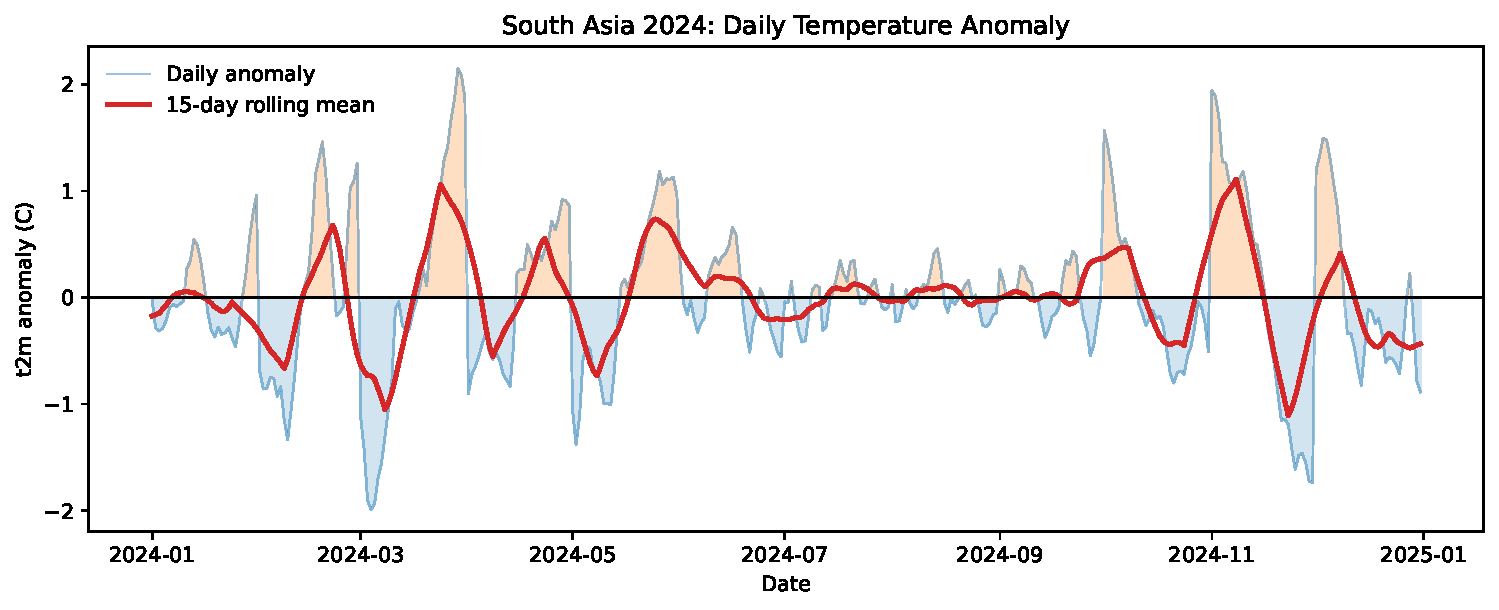
\includegraphics[width=0.85\textwidth]{../data/figures/contrib_brajesh/anomaly_temperature_timeseries.pdf}
    \caption{Daily temperature anomaly time series (South Asia, 2024).}
\end{figure}

\begin{figure}[h]
    \centering
    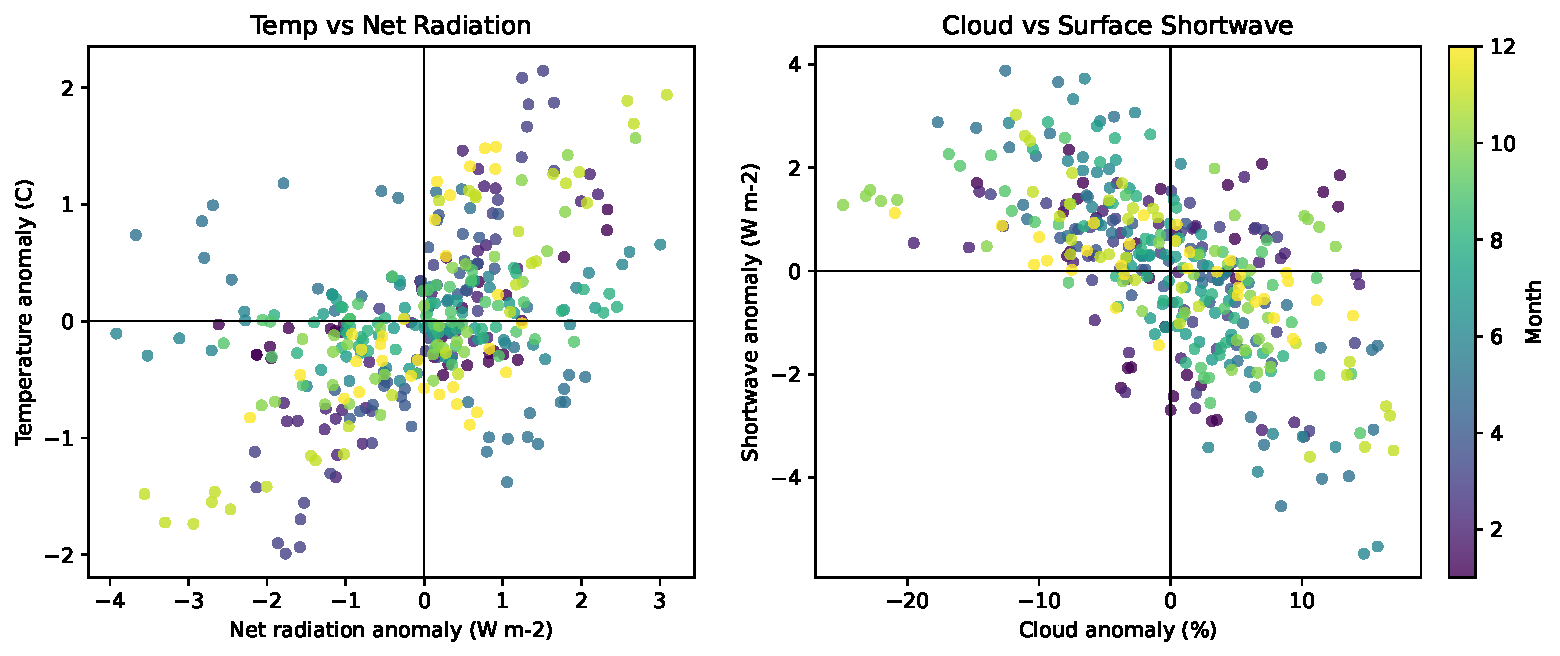
\includegraphics[width=0.85\textwidth]{../data/figures/contrib_brajesh/anomaly_relationships.pdf}
    \caption{Relationships among anomaly variables (temperature, cloud, and radiation).}
\end{figure}

\section{Conclusion and Outlook}
The assignment goals are largely satisfied: we built comparable Pandas and
Dask pipelines, benchmarked runtime and memory under multiple chunk settings,
and validated numerical consistency for both daily metrics and anomalies.

Key practical finding: on this hardware and workload, a well-optimized Pandas
pipeline can remain faster at this scale, while Dask provides safer scaling
headroom and better control over memory pressure as workload size grows.

Next steps include extending the Dask pipeline to additional global scenarios
and refining narrative discussion of observed scalability limitations.

\section{Acknowledgements}
We thank the course team for providing the report template and project
guidelines.

\section{Author Contributions}
All authors contributed to planning and implementation. Data acquisition,
baseline analysis, Dask workflow development, benchmarking, validation, and
report writing were completed collaboratively, with primary ownership divided
across team members by module.

\section{Code availability}
The code for this project is available at the following GitHub repository:
\url{https://github.com/dahiya-aditya/Dask-Pandas}.

% --------------------------------------------------------------------
% --------------------------------------------------------------------
% ---- DO NOT CHANGE THIS BLOCK OF CODE
\section{References}
\bibliography{refs}
% --------------------------------------------------------------------
% --------------------------------------------------------------------


\section{Appendix}

\subsection{Additional figures}
Additional outputs used during analysis include:
\begin{itemize}
    \item \verb|../data/figures/contrib_brajesh/anomaly_monthly_summary.pdf|
    \item \verb|../data/figures/contrib_brajesh/dask_annual_temperature_cycle.pdf|
    \item \verb|../data/figures/contrib_brajesh/dask_monthly_energy_budget.pdf|
\end{itemize}

\subsection{Algorithms}
The core reduction algorithm is implemented in code and validated by
Pandas-vs-Dask parity checks (35/35 checks passed under configured tolerances).


\subsection{Code snippets}
Code snippet showcase is intentionally omitted in this draft.


% --------------------------------------------------------------------
% --------------------------------------------------------------------
% ---- DO NOT CHANGE THIS BLOCK OF CODE
\end{document}
% --------------------------------------------------------------------
% --------------------------------------------------------------------
